\chapter{Calcul des déplacements}
Dans ce chapitre, nous allons commencer par écrire l'équation de la déformée 
pour quelques cas particuliers (et donc rares). Nous utiliserons ensuite notre 
nouveau théorème fétiche pour élaborer une méthode plus générale.

\section{Équation de la déformée}
	\subsection{Cf. titre de section (flemme)}
	Rappelons les équations obtenues lors de l'étude de la flexion simple\footnote{
	La première relation néglige les déplacements dus à l'effort tranchant.}
	\begin{itemize}
	\item[$\bullet$] Relation moment - courbure : $v'' = -\frac{M}{EI}$
	\item[$\bullet$] Relation $M-T$ (équilibre de rotation) : $\frac{dM}{dx}=T$
	\item[$\bullet$] Relation $T-q$ (équilibre de translation) : $\frac{dT}{dx}
	=-q(x)$
	\end{itemize}
	Les équations d'équilibres donnent 
	\begin{equation}
	\dfrac{d^2M}{dx^2} = \dfrac{dT}{dx},\qquad \dfrac{d^2M}{dx^2}=-q(x).
	\end{equation}
	On trouve alors (en dérivant deux fois)
	\begin{equation}
	v'' = -\dfrac{M}{EI} \longrightarrow \quad EIv'' = -M\longrightarrow \quad 
	(EIv'')'' = -\dfrac{d^2M}{dx^2}
	\end{equation}
	Comme $\dfrac{d^2M}{dx^2} = -q(x)$, on trouve pour le sections 
	\textbf{homogènes} ($E=E(x)$) :
	\begin{equation}
	(EIv'')'' = q(x)
	\end{equation}
	ou si j'ai carrément une \textbf{poutre homogène} (même chose dans toutes 
	les sections, $E =\ cste$) :
	\begin{equation}
	EIv^{(4)} = q(x)
	\end{equation}
	
	\subsection{Conditions aux limites}
	L'ED que nous venons d'obtenir est du quatrième ordre (youhou), il faut 
	donc quatre conditions aux limites (cf. \textit{Analyse II}) :
	\begin{enumerate}
	\item Sur $v$ (imposer la flèche, comme pour un appui)
	\item sur $v'$ (ça sera donc lié à $M$. Point au moment fléchissant nul : 
	$v''=0$, extrémité libre (encastrement))
	\item Sur $v''$ (moment fléchissant imposé)
	\item Sur $v'''$ (dérivée de \dots qui est la dérivée de $T$ : condition 
	sur l'effort tranchant (extrémité libre))(moment tranchant imposé)	
	\end{enumerate}
	\begin{center}
	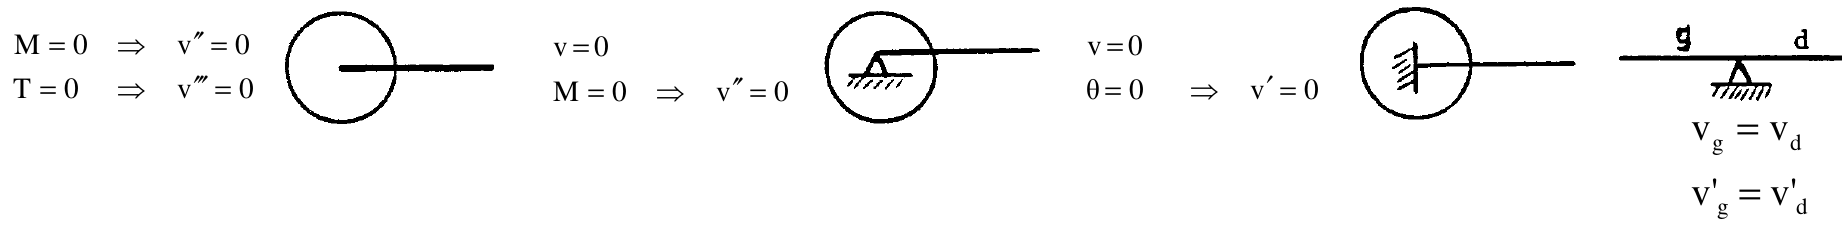
\includegraphics[scale=0.24]{ch9/image1}
	\captionof{figure}{ }
	\end{center}


\section{Théorèmes de travaux virtuels}
	\subsection{Travail virtuel pour des déplacements virtuels}
	On va à nouveau reconsidérer deux ensembles (virtuels et réels) et 
	reprendre la définition du travail virtuel total $T_{tot}' = 
	T_{ext}'+T_{int}'$, mais encore 
	\begin{equation}
	T_{tot}' \equiv \int_V f_iu_i'\ dV + \oint_S T_i^{(n)}u_i'\ dS - 
	\int_V \tau_{ij}a_{ij}'\ dV
	\label{eq:Approche}
	\end{equation}
		
		\subsubsection{Philosophie de l'approche}
		Toute la subtilité de la technique joue sur l'équivalence entre 
		\autoref{eq:Approche} et 
		\begin{equation}
		T_{tot}' \equiv \int_V(\tau_{ji,j}+f_i)u_i'\ dV +\oint_S (T_i^{(n)}
		-\tau_{ji}n_j)u_i'\ dS + \int_V \tau_{ji}u_{[i,j]}'\ dV
		\end{equation}
		
	\subsection{Théorèmes des TV pour des ensembles virtuels}
	Nous allons reprendre depuit le début en prenant cette fois deux 
	ensembles \textbf{virtuels} distincts :
	\begin{enumerate}
	\item Virtuel (') - déplacement : $u_i'$
	\item Virtuel ('') - forces de volume et de surface $f_i''\ dV\dots 
	T_i^{''(n)}\ dS$
	\end{enumerate}
	Reprenons le travail virtuel des forces extérieures : rien ne change, 
	il suffit de mettre des secondes partout
	\begin{equation}
	T_{ext}' \equiv \int_V f_i''u_i'\ dV + \oint_S T^{''(n)}u_i'\ dS
	\end{equation}
	On peut ainsi énoncer (et démontrer) le même théorèmes : il suffit 
	de mettre des secondes aux bons endroits. Le travail virtuel 
	intérieur et total se définit de façon similaire.\\
	
	Ces deux ensembles permettent de particulariser :
	\begin{enumerate}
	\item Déplacement réel \& forces virtuelles en équilibre $\rightarrow$ 
	pour calculer un déplacement réel.
	\item Déplacement virtuel \& forces réelles en équilibre $\rightarrow$ 
	pour calculer une force réelle.	
	\end{enumerate}
	
		\newpage
		\subsubsection{Exemple : calcul d'un déplacement}
		\begin{wrapfigure}[10]{r}{6.2cm}
		\vspace{-5mm}
		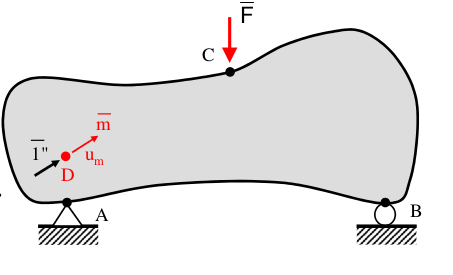
\includegraphics[scale=0.4]{ch9/image2.png}
		\captionof{figure}{ }
		\end{wrapfigure}	
		Considérons une patatoïde quelconque soumise à une force 
		quelconque sur laquelle j'identifie un point $D$. Sous l'effet de 
		tout ce qui est réel, ce point $D$ subit un déplacement $u$. On 
		s'intéresse à la composante de ce déplacement dans la direction 
		qui nous intéresse, à savoir $m$. Nous allons donc faire travailler 
		$u_m$ avec une force virtuelle.\\
		
		Pour se faire, considérons une force $\vec{1''}$ permettant de 
		trouver $u_m$. On pourrait dire "TV et équilibre : ma force vaut 
		1". Non, non et non : il faut considérer tout le tenseur qui va 
		équilibrer le bazar à l'intérieur mais aussi les réactions de 
		liaisons virtuelles qui équilibrent aussi le tout.
		Mais l'idée est bien la, il faut appliquer le TV pour des 
		déplacements réels et des forces virtuelles en équilibres. Ces 
		forces virtuelles en équilibres sont une force $1''$ équilibrée 
		selon $\vec{m}$ par les réactions de liaisons.\\
		Comme les déplacements réels ne sont pas infinitésimaux, il faut 
		considérer le théorème général.
		
		
	\subsection{Calcul d'un déplacement}
	Considérons le TV pour les déplacements réels
	\begin{equation}
	T_{tot}' \equiv \int_V f_i''u_i'\ dV + \oint_S T^{''(n)}u_i'\ dS - 
	\int_V \tau_{ij}''a_{ij}\ dV = 0
	\end{equation}
	Pour la force valant 1 au point $D$, le TV des forces extérieures se 
	réduit à 
	\begin{equation}
	T_{ext}' \equiv \int_V f_i''u_i'\ dV + \oint_S T^{''(n)}u_i'\ dS\qquad
	\Longrightarrow\qquad T_{ext}' = \vec{1''}.\vec{u} = \vec{u}.\vec{m}=u_m
	\end{equation}
	On a donc
	\begin{equation}
	u_m = \int_V \tau_{ij}''a_{ij}\ dV
	\end{equation}
	Il faut maintenant calculer $\tau_{ij}''$ et $a_{ij}$.
	
		\subsubsection{Exemple : les intégrales de Mohr}
		Grâce à la théorie des poutres, on peut calculer le déplacement 
		d'un point. On va calculer $u_m$ en fonction des contraintes de 
		la théorie des poutres :
		\begin{itemize}
		\item[$\bullet$] L'application des forces \textit{réelles} 
		(provoquant le déplacement recherché) donne une réparation de $M, 
		T$ et $N$.
		\item[$\bullet$] L’application de la force \textit{virtuelle} 
		auxiliaire donne une répartition de $M", T"$ et $N"$.
		\end{itemize}
		
	\newpage
	\subsection{Les intégrales de Mohr}
	Il faut calculer les contributions du moment fléchissant, de l'effort 
	normal et de l'effort tranchant. J'ai un peu la flemme\footnote{C'est la 
	dernière section de tout le cours, normal non?}, mais c'est pas 
	très dur : cf. slides 19-21.\\
	La contribution totale est obtenue en sommant ces différentes 
	contributions :
	\begin{equation}
	u_m = \int_{\Gamma} \dfrac{M"M}{EI}\ ds + \int_\Gamma \dfrac{N"N}{EA}\ ds + 
	\int_\Gamma	\chi\dfrac{T"T}{GA}\ ds
	\end{equation}
	où $\Gamma$ est la longueur de la poutre.\\
	\danger On peut sommer les contributions grâce au caractère 
	énergétiquement orthogonal des diagrammes $M, N, T$ (évident pour $M-N$ 
	et $T$). Ceci est démontré au slide 23.\\
	
	En bref : $M,N,T$ sont dus aux forces réellement appliquées à la structure 
	alors que $M", N", T"$ sont dus à une "force" unitaire appliquée au point 
	dont on cherche le déplacement, selon la ligne d'action et dans le sens de 
	ce déplacement\footnote{\danger On les note avec des ' ci dessous.}.\\
	
	Pour calculer ces intégrales, on utilise un tableau des combinaisons les 
	plus usuelles pour 
	\begin{equation}
	\dfrac{1}{L}\int_L M'M"\ dx
	\end{equation}
	\danger Ce tableau ne contient \textbf{pas} le facteur $1/EI$ à ne pas 
	oublier à l'examen. De plus, il ne faut pas oublier de multiplier par 
	$L$ à cause du $1/L$ sinon\dots\\
	
	Par contre, bonne nouvelle, ce tableau est aussi valable pour les couples 
	$N'N"$ et $T'T"$ (\danger avec le facteur $1/EA$).
	\begin{center}
	
\includegraphics[scale=0.4]{ch8/image3}
	\end{center}
		
